\section{Results and Discussion} \label{sec:results}

Here, we report a series of benchmarks that evaluate the viability of our proposed approaches to harness the CS-2 accelerator for digital evolution simulations and extract phylogenetic records from said simulations.
First, we compare the performance characteristics of new surface-oriented hereditary stratigraphy methods against preceding column-based implementation to determine the extent to which they succeed in streamlining runtime operations.
Then, we benchmark phylogeny-tracked WSE genetic algorithm implementations.
To assess the runtime overhead of surface-based tracking, we compare against benchmarking results with phylogenetic tracking disabled.
Finally, we validate the credibility of the presented end-to-end annotation-to-reconstruction pipeline by reviewing clade structure and phylometric properties from emulated and on-hardware runs.

\subsection{Surface Algorithm Benchmark on Conventional CPU}

\begin{figure*}
  \centering
  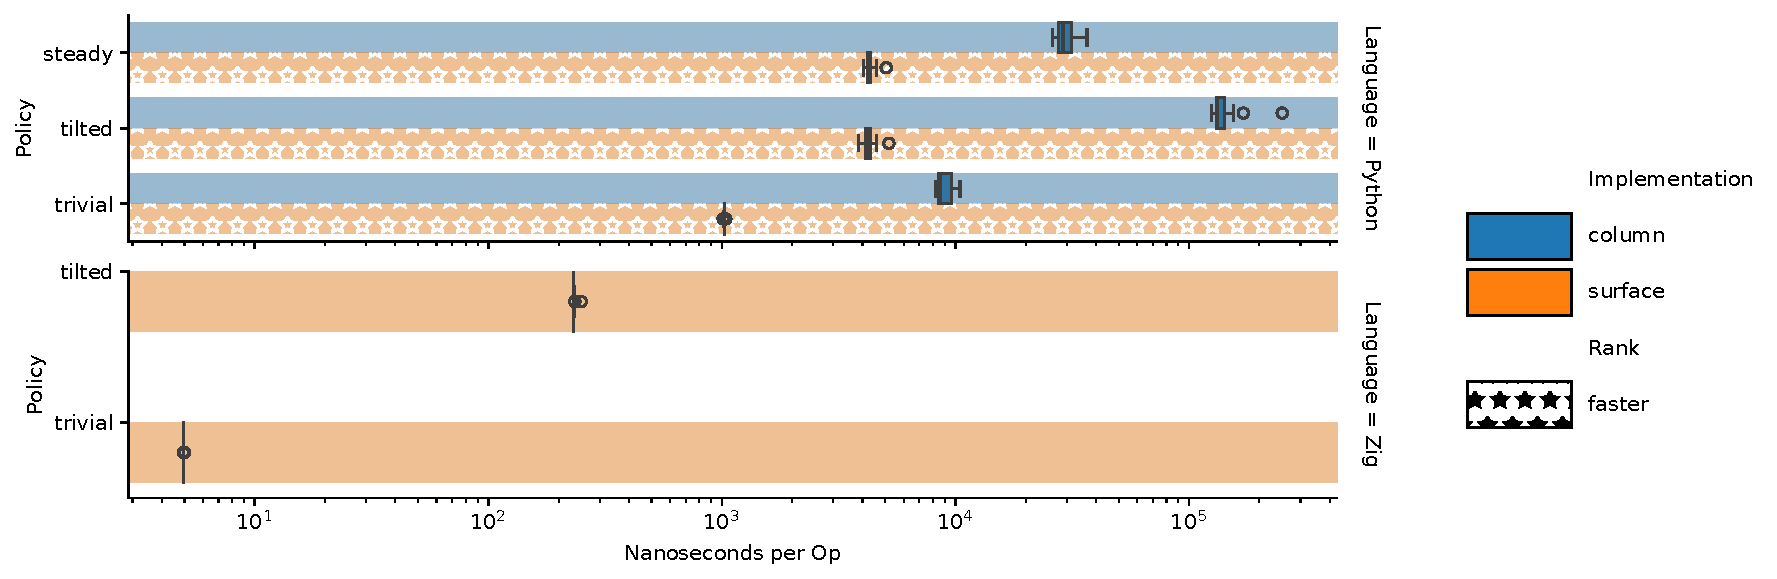
\includegraphics[width=0.85\textwidth,trim={0 0 0 0.4in
  }, clip]{binder-wafer-scale/binder/teeplots/all=false+hue=implementation+orient=h+row=language+score=nanoseconds-per-op+viz=peckplot+x=nanoseconds-per-op+y=policy+y-group=outer+ext=}

\vspace{-2.5ex}

  \caption{%
    \textbf{Hereditary stratigraphy algorithm benchmarks.}
    \footnotesize
    Comparison of per-generation operation time for column- and surface-based steady and tilted retention policies, lower is better.
  Top and bottom panels show Python and Zig implementations, respectively.
    Trivial is a simple harcoded retention decision, provided as a baseline control.
    Background hatching indicates significant outcome (Mann-Whitney U test; $n=20$).
  }
  \label{fig:benchmarking}
  \vspace{-0.2in}
\end{figure*}


We performed microbenchmark experiments to test computational efficiency of new surface-based algorithms.
Trials measured the real-time speed of sequential generation updates on one annotation with capacity for 64 differentiae.
Benchmarks used both Python, for comparability with existing column algorithm implementations, and Zig, to assess performance under compiler optimization.
Figure \ref{fig:benchmarking} overviews results.

% https://github.com/mmore500/hstrat-surface-concept/blob/51d636d768d474fc5148b9fcaa199c1b7776e915/benchmark.ipynb
Python implementations of the surface tilted and steady algorithms both took around 4.2 microseconds per operation (standard errors [SE] 50ns and 66ns; $n=20$).
For context, this speed was about $4\times$ the measured time for a surface placement using a trivial calculation (SE 0.05; $n=20$).
As expected, column implementations of steady and tilted fared much worse, taking about $7\times$ and $34\times$ the execution time per operation compared to the surface operations.
In both cases, surface implementations significantly outperformed their column counterparts (Mann-Whitney U test, $\alpha = 0.05$).
% While Python is an interpreted language and the Python-implemented algorithms weren't specifically implemented to maximize performance and suffer an intrinsic performance penalty due to that, the algorithms were all on the same footing and
% We use the ``optimize''' flag to strip superfluous safety checks.

% https://github.com/mmore500/wse-sketches/blob/d42e9174025bc67fa669347611d1a82b9ea5843c/binder/benchmark.ipynb
Zig microbenchmarks clock tilted surface annotation updates at 230 ns per operation (SE 0.9ns; $n=20$).
For context, this time is a little more than twice that required for a main memory access in contemporary computing hardware \citep{markus2022memory}.
Our results measure the operation at $49\times$ the measured time for a trivial placement calculation (SE 0.03; $n=20$).
Zig steady implementation clocks 511 ns per operation (SE 4; $n=20$), $110\times$ trivial (SE 0.8ns; $n=20$).
Note that speedup of Zig implementations relative to Python reflects an intrinsic performance penalty due to interpreter overhead of Python evaluation.
However, comparisons among Python implementations and among Zig implementations are nonetheless informative because all are on equal footing in this regard.

% \footnote{Steady results are not included, due to a Zig implementation not yet being completed.}

Low-hanging speedups and optimizations exist to further improve the per-operation surface update performance achieved in practice.
Half of update operations on surfaces with single-bit differentiae can be skipped entirely, owing to 50\% probability that randomization fails to change a stored differentia value.
Further, simulations with synchronous or near-synchronous generations can cache calculated surface-placement indices, meaning they would only need to be computed once for an entire subpopulation.
Another possibility is to coarsen temporal resolution, only updating annotations at intervals every $n$th generation.

\subsection{Wafer-Scale Engine Island-model GA Benchmark}

Next, we used an emulator to characterize the expected performance of our island model genetic algorithm on WSE hardware and estimate the magnitude of simulation that might be achieved with on-device execution.
We used the emulator's per-PE clock cycle counters to measure the amount of real time elapsed over the course of a 40-generation-cycle simulation.
We tested using a $3\times3$ PE collective with the tagged 3-word genome and a per-PE population size of 32, applying a tilted hereditary stratigraphy every generation.
PEs completed a mean of 24,138 generation cycles per second (SEM 99; $n=9$).
As an indicator of inter-PE exchange throughput, each PE immigrated a mean of 118 genomes (SEM 11; $n=9$) over 40 elapsed generation cycles.

% https://osf.io/tf89g
What scale of simulation does this performance imply at full scale on CS-2 hardware?
Across eight on-device, tracking-enabled trials of 1 million generations (described in the following section), we measured a mean simulation rate of 17,688 generations per second for 562,500 PEs ($750\times750$ rectangle) with run times slightly below one minute.
Trials with 1,600 PEs ($40\times40$) performed similarly, completing 17,734 generations per second.

Multiplied out to a full day, 17 generations per second turnover would elapse around 1.5 billion generations.
With 32 individuals hosted per each of 850,000 PEs, the net population size would sit around 27 million at full CS-2 wafer scale.
(Note, though, that available on-chip memory could support thousands of our very simple agents per PE, raising the potential for a net population size on the order of a billion agents.)
% 24,000 * 850,000 * 60 * 60 * 24 * 32 ---> ?? quadrillion
A naive extrapolation estimates on the order of a quadrillion agent replications could be achieved hourly at full wafer scale for such a very simple model.
We look forward to conducting more thorough benchmarking and scaling experiments in future work.
%The barebones simplicity of the model should also be noted.

How fast is simulation without hstrat instrumentation?
We repeated our hardware-emulated benchmark with 32-bit genomes stripped of all instrumentation.
Under these conditions, PEs completed on average 47,175 generations per second (SEM 220; $n=9$) and immigrated 118 genomes (SEM 12; $n=9$).

These timings indicate cost of phylogeny tracking is approximately equivalent to that of the other aspects of simulation, combined.
Given the highly minimalistic nature of the agent model and selection process, this result is highly promising.
In actual use, most experiments will likely involve a much more sophisticated agent model; thus, the relative overhead of tracking will diminish significantly.
It is additionally worthwhile to note that caching and coarsening strategies discussed above have not yet been applied, which may reduce the performance penalty of tracking considerably.

% https://github.com/mmore500/wse-sketches-mirror/actions/runs/8590107511/job/23537207835
% from https://github.com/mmore500/wse-sketches-mirror/commit/3a1bf8e9f2820a38cb7387a7624a86361485174b
% ASYNC_GA_GENOME_FLAVOR genome_purifyingplus
% ASYNC_GA_GLOBAL_SEED 0
% ASYNC_GA_NCYCLE_AT_LEAST 40
% ASYNC_GA_MSEC_AT_LEAST 0
% ASYNC_GA_TSC_AT_LEAST 0
% INFO: Using SIF: /home/runner/cerebras/bin/cbcore_sdk-202311111408-10-4a54bce5.sif
% INFO: User's specified CSL_IMPORT_PATH=
% NOTE: CSL_IMPORT_PATH accepts colon separated list of paths generated by 'realpath <path>'
% INFO:    Environment variable SINGULARITYENV_CSL_SUPPRESS_SIMFAB_TRACE is set, but APPTAINERENV_CSL_SUPPRESS_SIMFAB_TRACE is preferred
% compile successful
% Updated 1 path from the index
% CS_PYTHON cs_python
% INFO: Using SIF: /home/runner/cerebras/bin/cbcore_sdk-202311111408-10-4a54bce5.sif
% INFO:    Environment variable SINGULARITYENV_CSL_SUPPRESS_SIMFAB_TRACE is set, but APPTAINERENV_CSL_SUPPRESS_SIMFAB_TRACE is preferred
% whoami ===============================================================
% [[0 3 6]
%  [1 4 7]
%  [2 5 8]]
% whereami x ===========================================================
% [[0 1 2]
%  [0 1 2]
%  [0 1 2]]
% whereami y ===========================================================
% [[0 0 0]
%  [1 1 1]
%  [2 2 2]]
% cycle counter =======================================================
% [[40 40 40]
%  [40 40 40]
%  [40 40 40]]
% recv counter N ========================================================
% [[ 1  1  1]
%  [ 9 13 11]
%  [15 12 12]]
% recv counter S ========================================================
% [[ 7  9  8]
%  [10 11  9]
%  [ 1  1  1]]
% recv counter E ========================================================
% [[12 11  1]
%  [12 13  1]
%  [ 9 13  1]]
% recv counter W ========================================================
% [[ 1 11  9]
%  [ 1  7  9]
%  [ 1 10 11]]
% recv counter sum =====================================================
% [21, 32, 19, 32, 44, 30, 26, 36, 25]
% np.mean(recvSum)=29.444444444444443 np.std(recvSum)=7.304657739508267 sps.sem(recvSum)=2.5825865109265465
% send counter N ========================================================
% [[ 0  0  0]
%  [24 32 34]
%  [40 46 34]]
% send counter S ========================================================
% [[38 50 46]
%  [58 50 48]
%  [ 0  0  0]]
% send counter E ========================================================
% [[44 32  0]
%  [24 32  0]
%  [40 46  0]]
% send counter W ========================================================
% [[ 0 50 46]
%  [ 0 50 48]
%  [ 0 36 48]]
% send counter sum =====================================================
% [82, 132, 92, 106, 164, 130, 80, 128, 82]
% np.mean(sendSum)=110.66666666666667 np.std(sendSum)=27.744869395579748 sps.sem(sendSum)=9.809292646374773
% tscControl values ====================================================
% [30064968187, 30064968187, 30064968187, 30064968187, 30064968187, 30064968187, 30064968187, 30064968187, 30064968187]
% tscStart values ======================================================
% [2220, 2222, 2731, 2731, 1716, 2738, 3241, 3243, 3237]
% tscEnd values ========================================================
% [1414233, 1414662, 1406657, 1388294, 1438771, 1433887, 1412082, 1403426, 1390454]
% tsc diffs ============================================================
% --------------------------------------------------------------- ticks
% [1412013, 1412440, 1403926, 1385563, 1437055, 1431149, 1408841, 1400183, 1387217]
% np.mean(tsc_ticks)=1408709.6666666667 np.std(tsc_ticks)=16415.157825754963 sps.sem(tsc_ticks)=5803.63470641938
% -------------------------------------------------------------- seconds
% [0.0016611917647058824, 0.0016616941176470588, 0.0016516776470588235, 0.0016300741176470588, 0.0016906529411764705, 0.0016837047058823528, 0.00165746, 0.0016472741176470588, 0.00163202]
% np.mean(tsc_sec)=0.0016573054901960784 np.std(tsc_sec)=1.9311950383241098e-05 sps.sem(tsc_sec)=6.827805536963963e-06
% ---------------------------------------------------- seconds per cycle
% [4.152979411764706e-05, 4.154235294117647e-05, 4.129194117647059e-05, 4.075185294117647e-05, 4.226632352941176e-05, 4.209261764705882e-05, 4.1436499999999995e-05, 4.1181852941176466e-05, 4.0800500000000003e-05]
% np.mean(tsc_cysec)=4.143263725490196e-05 np.std(tsc_cysec)=4.827987595810268e-07 sps.sem(tsc_cysec)=1.7069513842409884e-07
% ---------------------------------------------------------- cycle hertz
% [24079.09842189838, 24071.81897992127, 24217.800653310787, 24538.761499837972, 23659.498070707108, 23757.135001317125, 24133.312417795907, 24282.540210815303, 24509.50356000539]
% np.mean(tsc_cyhz)=24138.829868401026 np.std(tsc_cyhz)=280.43062795032466 sps.sem(tsc_cyhz)=99.14719933803819
% --------------------------------------------------------- ns per cycle
% [41529.79411764706, 41542.35294117647, 41291.94117647059, 40751.852941176476, 42266.32352941176, 42092.61764705882, 41436.49999999999, 41181.85294117647, 40800.5]
% np.mean(tsc_cyns)=41432.63725490196 np.std(tsc_cyns)=482.7987595810264 sps.sem(tsc_cyns)=170.6951384240987
% fitness =============================================================
% [[0.00316905 0.00565182 0.0022315 ]
%  [0.00687918 0.00742484 0.00589414]
%  [0.00582986 0.0057458  0.00379858]]


% https://github.com/mmore500/wse-sketches-mirror/actions/runs/8590107511/job/23537207835
% from https://github.com/mmore500/wse-sketches-mirror/commit/3a1bf8e9f2820a38cb7387a7624a86361485174b
% CSLC cslc
% ASYNC_GA_GENOME_FLAVOR genome_purifyingstripped
% ASYNC_GA_GLOBAL_SEED 0
% ASYNC_GA_NCYCLE_AT_LEAST 40
% ASYNC_GA_MSEC_AT_LEAST 0
% ASYNC_GA_TSC_AT_LEAST 0
% INFO: Using SIF: /home/runner/cerebras/bin/cbcore_sdk-202311111408-10-4a54bce5.sif
% INFO: User's specified CSL_IMPORT_PATH=
% NOTE: CSL_IMPORT_PATH accepts colon separated list of paths generated by 'realpath <path>'
% INFO:    Environment variable SINGULARITYENV_CSL_SUPPRESS_SIMFAB_TRACE is set, but APPTAINERENV_CSL_SUPPRESS_SIMFAB_TRACE is preferred
% compile successful
% Updated 1 path from the index
% CS_PYTHON cs_python
% INFO: Using SIF: /home/runner/cerebras/bin/cbcore_sdk-202311111408-10-4a54bce5.sif
% INFO:    Environment variable SINGULARITYENV_CSL_SUPPRESS_SIMFAB_TRACE is set, but APPTAINERENV_CSL_SUPPRESS_SIMFAB_TRACE is preferred
% whoami ===============================================================
% [[0 3 6]
%  [1 4 7]
%  [2 5 8]]
% whereami x ===========================================================
% [[0 1 2]
%  [0 1 2]
%  [0 1 2]]
% whereami y ===========================================================
% [[0 0 0]
%  [1 1 1]
%  [2 2 2]]
% cycle counter =======================================================
% [[40 40 40]
%  [40 40 40]
%  [40 40 40]]
% recv counter N ========================================================
% [[ 1  1  1]
%  [13 11 14]
%  [11  7 11]]
% recv counter S ========================================================
% [[ 9 13  9]
%  [11 13 11]
%  [ 1  1  1]]
% recv counter E ========================================================
% [[11 15  1]
%  [ 7 11  1]
%  [ 7  9  1]]
% recv counter W ========================================================
% [[ 1  7  9]
%  [ 1  9 13]
%  [ 1 11 13]]
% recv counter sum =====================================================
% [22, 36, 20, 32, 44, 39, 20, 28, 26]
% np.mean(recvSum)=29.666666666666668 np.std(recvSum)=8.16496580927726 sps.sem(recvSum)=2.886751345948129
% send counter N ========================================================
% [[ 0  0  0]
%  [38 52 38]
%  [42 52 44]]
% send counter S ========================================================
% [[54 44 56]
%  [44 30 44]
%  [ 0  0  0]]
% send counter E ========================================================
% [[28 38  0]
%  [38 52  0]
%  [42 52  0]]
% send counter W ========================================================
% [[ 0 44 56]
%  [ 0 30 44]
%  [ 0 30 38]]
% send counter sum =====================================================
% [82, 126, 112, 120, 164, 126, 84, 134, 82]
% np.mean(sendSum)=114.44444444444444 np.std(sendSum)=26.192073063391234 sps.sem(sendSum)=9.260296238228726
% tscControl values ====================================================
% [30064968187, 30064968187, 30064968187, 30064968187, 30064968187, 30064968187, 30064968187, 30064968187, 30064968187]
% tscStart values ======================================================
% [1131, 1130, 1644, 1641, 628, 1650, 2151, 2155, 2149]
% tscEnd values ========================================================
% [709983, 736796, 714836, 730020, 721384, 731436, 713213, 730922, 713242]
% tsc diffs ============================================================
% --------------------------------------------------------------- ticks
% [708852, 735666, 713192, 728379, 720756, 729786, 711062, 728767, 711093]
% np.mean(tsc_ticks)=720839.2222222222 np.std(tsc_ticks)=9500.522988853212 sps.sem(tsc_ticks)=3358.9421151183965
% -------------------------------------------------------------- seconds
% [0.0008339435294117647, 0.0008654894117647059, 0.0008390494117647059, 0.0008569164705882353, 0.0008479482352941177, 0.0008585717647058823, 0.0008365435294117647, 0.0008573729411764705, 0.00083658]
% np.mean(tsc_sec)=0.0008480461437908496 np.std(tsc_sec)=1.1177085869239065e-05 sps.sem(tsc_sec)=3.9516966060216395e-06
% ---------------------------------------------------- seconds per cycle
% [2.0848588235294117e-05, 2.1637235294117648e-05, 2.097623529411765e-05, 2.1422911764705883e-05, 2.119870588235294e-05, 2.1464294117647056e-05, 2.0913588235294118e-05, 2.1434323529411762e-05, 2.0914499999999998e-05]
% np.mean(tsc_cysec)=2.1201153594771243e-05 np.std(tsc_cysec)=2.7942714673097676e-07 sps.sem(tsc_cysec)=9.879241515054106e-08
% ---------------------------------------------------------- cycle hertz
% [47964.878423140515, 46216.62547949749, 47672.99689284232, 46678.995413102246, 47172.6908967806, 46589.00006303218, 47815.80227884488, 46654.14323096409, 47813.71775562409]
% np.mean(tsc_cyhz)=47175.427825980936 np.std(tsc_cyhz)=620.9035009060691 sps.sem(tsc_cyhz)=219.52253797657457
% --------------------------------------------------------- ns per cycle
% [20848.58823529412, 21637.235294117647, 20976.23529411765, 21422.91176470588, 21198.70588235294, 21464.294117647056, 20913.58823529412, 21434.323529411762, 20914.499999999996]
% np.mean(tsc_cyns)=21201.15359477124 np.std(tsc_cyns)=279.42714673097595 sps.sem(tsc_cyns)=98.79241515054076
% fitness =============================================================
% [[0. 0. 0.]
%  [0. 0. 0.]
%  [0. 0. 0.]]

\subsection{Clade Reconstruction Trial}

Here, we demonstrate phylogenetic reconstructions from emulated WSE hardware and inspect clade structure to qualitatively assess their credibility.
For these experiments, we tagged genomes with a 16-bit randomly generated identifier at simulation startup, as shown in Supplementary Figure \ref{fig:genome-layout} \citep{moreno2024supplement}.
Using the hardware emulator, we instantiated populations over a $3\times3$ PE collective for durations of 25, 50, 100, and 250 generation cycles under drift conditions.
At the end of simulation, phylogenetic reconstruction was conducted using one genome sampled per PE.

\begin{figure}

\begin{subfigure}[c]{\linewidth} \centering
\begin{minipage}[c]{0.08\linewidth} \flushright
    \caption{\rotatebox[origin=c]{90}{25 cycles}}
    \label{fig:tagged_25}
  \end{minipage}%
  \begin{minipage}[c]{0.92\linewidth}
    \includegraphics[width=\textwidth,height=0.6in,trim={0 0.81cm 0 0},clip]{binder-wse-sketches/binder/teeplots/genome=hsurftiltedsticky_tagged+replicate=e4ea2071-8228-42de-af8c-879cedff9ba7+viz=draw-biopython-tree+ext=}
  \end{minipage}%
\end{subfigure}

\vspace{-1ex}

\begin{subfigure}[c]{\linewidth} \centering
\begin{minipage}[c]{0.08\linewidth} \flushright
    \caption{\rotatebox[origin=c]{90}{50 cycles}}
    \label{fig:tagged_50}
  \end{minipage}%
  \begin{minipage}[c]{0.92\linewidth}
    \includegraphics[width=\textwidth,height=0.6in,trim={0 0.81cm 0 0},clip]{binder-wse-sketches/binder/teeplots/genome=hsurftiltedsticky_tagged+replicate=3d55af5f-7714-45da-9276-e860f46b4d94+viz=draw-biopython-tree+ext=}
  \end{minipage}%
\end{subfigure}

\vspace{-1ex}

\begin{subfigure}[c]{\linewidth} \centering
  \begin{minipage}[c]{0.08\linewidth} \flushright
    \caption{\rotatebox[origin=c]{90}{100 cycles}}
    \label{fig:tagged_100}
  \end{minipage}%
  \begin{minipage}[c]{0.92\linewidth}
    \includegraphics[width=\textwidth,height=0.6in,trim={0 0.81cm 0 0},clip]{binder-wse-sketches/binder/teeplots/genome=hsurftiltedsticky_tagged+replicate=932aa302-becb-47e8-9712-7f550b02364c+viz=draw-biopython-tree+ext=}
  \end{minipage}%
\end{subfigure}

\vspace{-1ex}

\begin{subfigure}[c]{\linewidth} \centering
  \begin{minipage}[c]{0.08\linewidth} \flushright
    \caption{\rotatebox[origin=c]{90}{250 cycles}}
    \label{fig:tagged_250}
  \end{minipage}%
  \begin{minipage}[c]{0.92\linewidth}
    \includegraphics[width=\textwidth,height=0.8in]{binder-wse-sketches/binder/teeplots/genome=hsurftiltedsticky_tagged+replicate=42dbcbb3-b803-41a4-9285-4a450bfad6ed+viz=draw-biopython-tree+ext=}
  \end{minipage}%
\end{subfigure}

\caption{%
\textbf{Clade Validation Trial.}
\footnotesize
Example phylogenies reconstructed from runs of increasing duration on virtual grid of nine hardware-simulated PEs.
Founding genomes were tagged with random 16-byte identifier values, which were held constant over the course of simulation (Supplementary Figure \ref{fig:genome-layout}).
Color-coding indicates each sampled taxon's founding ancestor according to this identifier value.
Simulation performed under drift conditions.
}
\label{fig:tagged}

\end{figure}


Figure \ref{fig:tagged} shows reconstructed phylogenies from each duration.
As expected, taxa belonging to the same founding clade (shown by color) are reconstructed as more closely related to each other than to other taxa.
Additionally, and also as expected, the number of distinct remaining founding clades diminishes monotonically with increasing simulation duration.
These consistencies corroborate the general integrity of implemented annotation and reconstruction processes.
Note, however, the incidence of moderate overestimations for relatedness between independently-tagged clades throughout.
As mentioned earlier, and discussed in greater depth elsewhere \citep{moreno2024guide}, this is an expected artifact of hereditary stratigraphy with single-bit differentia.
Applications requiring greater reconstruction precision can opt for larger differentia sizes and/or higher differentia counts.

\subsection{On-hardware Trial}

\begin{figure}

\begin{subfigure}[c]{\linewidth}
  \centering
    \includegraphics[width=0.9\linewidth]{binder-wse-sketches/binder/teeplots/col=metric+hue=regime+kind=swarm+post=teed-set-titles-col-name+viz=catplot+x=num-pes-10k+y=value+ext=}
    \vspace{-1.5ex}
 \caption{\footnotesize adaptive vs. purifying phylometric structure}
  \label{fig:on-device-phylometrics}
\end{subfigure}

\vspace{0.2ex}

\begin{subfigure}[c]{0.5\linewidth}
  \centering
  \includegraphics[width=0.7\linewidth,trim={0 11.05in 7.2in 0in},clip]{binder-wse-sketches/binder/outplots/linear/genomeFlavor=genome_purifyingplus+globalSeed=1.0+nCycle=1000000.0+popSize=562500+replicate=0d82d64b-991d-455b-84d8-cdf9edaad99d+ext=}

  \vspace{-2ex}
  \includegraphics[width=0.7\linewidth,trim={0 11.05in 7.2in 0in},clip]{binder-wse-sketches/binder/outplots/log/genomeFlavor=genome_purifyingplus+globalSeed=1.0+nCycle=1000000.0+popSize=562500+replicate=0d82d64b-991d-455b-84d8-cdf9edaad99d+ext=}

  \vspace{-3.5ex}
  \footnotesize
 \caption{\footnotesize adaptive regime}
  \label{fig:on-device-adaptive}
\end{subfigure}%
\begin{subfigure}[c]{0.5\linewidth}
  \centering
  \includegraphics[width=0.7\linewidth,trim={0 11.05in 7.2in 0in},clip]{binder-wse-sketches/binder/outplots/linear/genomeFlavor=genome_purifyingonly+globalSeed=1.0+nCycle=1000000.0+popSize=562500+replicate=ce2a0bf2-e132-4a61-95ec-c6ca54213949+ext=}

  \vspace{-2ex}
  \includegraphics[width=0.7\linewidth,trim={0 11.05in 7.2in 0in},clip]{binder-wse-sketches/binder/outplots/log/genomeFlavor=genome_purifyingonly+globalSeed=1.0+nCycle=1000000.0+popSize=562500+replicate=ce2a0bf2-e132-4a61-95ec-c6ca54213949+ext=}

  \vspace{-3.5ex}
  \footnotesize
 \caption{\footnotesize purifying regime}
  \label{fig:on-device-purifying}
\end{subfigure}

\vspace{-1.5ex}

\caption{%
\textbf{On-hardware Trial.}
\footnotesize
Results from phylogenetic reconstruction of 1 million generation on-hardware simulations.
Panel \ref{fig:on-device-phylometrics} compares phylometric readings from purifying-only and adaptation-enabled configurations, 4 replicates each.
Panels \labelcref{fig:on-device-adaptive,fig:on-device-purifying} juxtapose example $750\times750$ PE simulation phylogenies under each configuration regime.
Phylometrics were calculated from reconstructions with 10k sampled end-state agents.
For legibility, phylogeny visualizations were further subsampled to 1k end-state agents.
Top phylogenies are linear-scaled.
Bottom phylogenies are log-scaled with ultrametric correction to better show topology.
}
\label{fig:on-device}
\vspace{-0.2in}
\end{figure}


Finally, we set out to assess the performance of our pipeline at full wafer scale.
For these experiments, we used the four-word, tracking-enabled genome layout, with the full first 32 bits containing a floating point fitness value.
We defined two treatments: \textit{purifying-only}, where 33\% of agent replication events decreased fitness by a normally-distributed amount,  and \textit{adaption-enabled}, which added beneficial mutations that increased fitness by a normally-distributed amount, occurring with 0.3\% probability.
These beneficial mutations introduced the possibility for selective sweeps.
As before, we used tournament size 5 for both treatments.
We performed four on-hardware replicates of each treatment instantiated on 10k ($100\times100$), 250k ($500\times500$) and 562.5k ($750\times750$) PE arrays.
We halted each PE after it elapsed 1 million generations.

Upon completion, we sampled one genome from each PE.
Then, we performed an agglomerative trie-based reconstruction from subsamples of 10k end-state genomes \citep{moreno2024analysis}.
Figure \ref{fig:on-device} compares phylogenies generated under the purifying-only and adaption-enabled treatments.
As expected \citep{moreno2023toward}, purifying-only treatment phylogenies consistently exhibited greater sum branch length and mean evolutionary distinctiveness, with the effect on branch length particularly strong.
These structural effects are apparent in example phylogeny trees from 562.5k PE trials (Figures \labelcref{fig:on-device-adaptive,fig:on-device-purifying}).
Successful differentiation between treatments is a highly promising outcome.
This result not only supports the correctness of our methods and implementation, but also confirms the capability of reconstruction-based analyses to meaningfully describe dynamics of very large-scale evolution simulations.
